\documentclass[tikz, border=2pt]{standalone}
\usepackage[utf8]{inputenc}
\usepackage{tikz}
\usetikzlibrary{bayesnet}
\begin{document}
% \author{Karm Patel}
% \date{July 2022}
% \maketitle
\tikzstyle{constant} = [circle, draw=black!0, minimum size = 4mm]

\tikzstyle{det} = [circle, double, thick, draw=black!75, fill=gray!20, minimum size=4mm]
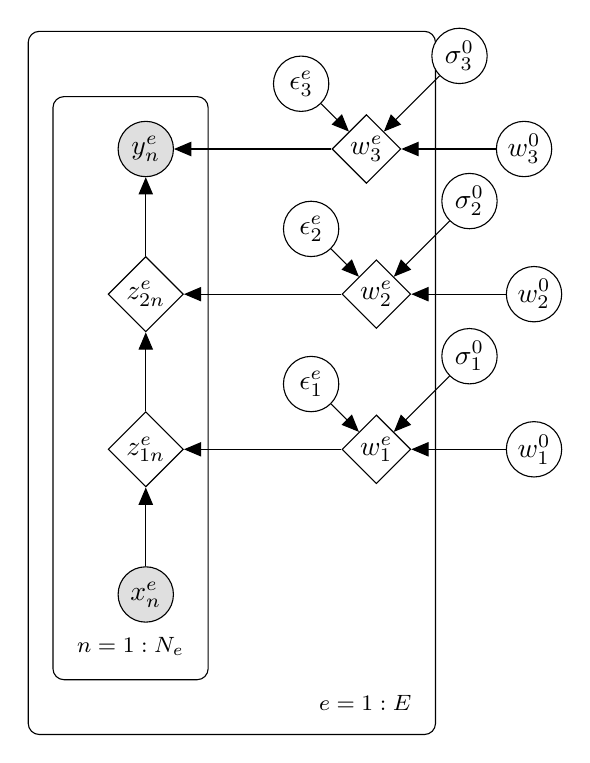
\begin{tikzpicture}
    \node [obs](y_n){$y_{n}^e$};
    \node [det, below= of y_n](z2_n){$z_{2n}^e$};
    \edge{z2_n}{y_n};
    \node [det, below= of z2_n](z1_n){$z_{1n}^e$};
    \edge{z1_n}{z2_n};
	\node [obs, below= of z1_n](x_n){$x_{n}^e$};
	\edge{x_n}{z1_n};
	\plate[inner sep=.3cm]{plate_inner}{(y_n)(z1_n)(z2_n)(x_n)}{$n=1:N_{e}$};
	
	\node [det, right=2cm of y_n](w3){$w_{3}^e$};
	\node [latent, above left= 0.5cm of w3](e3){$\epsilon_{3}^e$};
    \edge{e3}{w3};
    \edge{w3}{y_n}
    
    \node [det, right=2cm of z2_n](w2){$w_{2}^e$};
	\node [latent, above left= 0.5 cm of w2](e2){$\epsilon_{2}^e$};
    \edge{e2}{w2};
    \edge{w2}{z2_n}
    
    \node [det, right=2cm of z1_n](w1){$w_{1}^e$};
	\node [latent, above left= 0.5 cm of w1](e1){$\epsilon_{1}^e$};
    \edge{e1}{w1};
    \edge{w1}{z1_n}
    
    \plate[inner sep=.3cm]{plate_outer}{(plate_inner)(e3)(w1)(w2)(w3)}{$e=1:E$};
    
    \node [latent, above right=1cm of w3](sigma3){$\sigma_{3}^0$};
    \node[latent, right=1.2cm of w3](w30){$w_{3}^0$};
    \edge{sigma3}{w3}
    \edge{w30}{w3}
    
    \node [latent, above right=1cm of w2](sigma2){$\sigma_{2}^0$};
    \node[latent, right=1.2cm of w2](w20){$w_{2}^0$};
    \edge{sigma2}{w2}
    \edge{w20}{w2}
    
     \node [latent, above right=1cm of w1](sigma1){$\sigma_{1}^0$};
    \node[latent, right=1.2cm of w1](w10){$w_{1}^0$};
    \edge{sigma1}{w1}
    \edge{w10}{w1}
    
    

\end{tikzpicture}
\end{document}
